This system contains the video encoding subsystem, video rendering subsystem, and the head tracking translation subsystem. The subsystems communicate with the Camera System and the Virtual Reality System respectively. Video data will be received from the Camera System and rendered to the Virtual Reality System. The raw head tracking data is captured and translated to analog signals for the Camera System.

\begin{figure}[h!]
	\centering
 	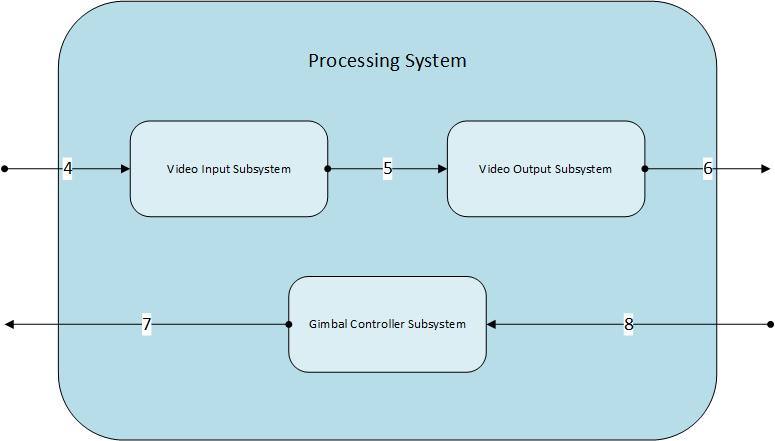
\includegraphics[width=0.60\textwidth]{images/processingsubsystem}
 \caption{Processing System Layer subsystem description diagram}
\end{figure}

\subsection{Layer Hardware}
A computer powerful enough to encode and render two 1080p 30 frames per second video, an Intel i5 or an Nvidia GeForce GTX 970 are the suggested minimums, and an Arduino Uno is used as the serical interface for the Storm32-BGC gimbal controller.

\subsection{Layer Operating System}
The supported operating system is Windows 7 or newer.

\subsection{Layer Software Dependencies}
An Oculus Rift setup utility has been executed on the computer. Unity 5.5 if cameras need to be adjusted or changes are needed. Arduino IDE is recommended if serial interface changes must be made as well as for the initial setup of the Arduino Uno.

\subsection{Video Encoding Subsystem}
This subsystem receives the raw FMPEG video streams from the Camera System. The raw video is encoded into a Unity texture.

\subsubsection{Subsystem Hardware}
A minimum of Intel i5 or Nvidia GeForce GTX 970 is suggested.

\subsubsection{Subsystem Operating System}
Windows 7 or newer

\subsubsection{Subsystem Software Dependencies}
Unity 5.5

\subsubsection{Subsystem Programming Languages}
C\# has been used as the default scripting language for its nativity in Unity.

\subsubsection{Subsystem Data Structures}
Array of textures and video frame buffers.

\subsubsection{Subsystem Data Processing}
FMPEG to Unity texture

\subsection{Video Rendering Subsystem}
This subsystem takes the two video textures and overlays them onto a user interface menu element. Then, the images are barreled and merged. The rendered image is streamed to the Virtual Reality System.

\subsubsection{Subsystem Hardware}
A minimum of Intel i5 or Nvidia GeForce GTX 970 is suggested.

\subsubsection{Subsystem Operating System}
Windows 7 or newer

\subsubsection{Subsystem Software Dependencies}
Unity 5.5

\subsubsection{Subsystem Programming Languages}
C\#

% Anything?
\subsubsection{Subsystem Data Structures}
None

\subsubsection{Subsystem Data Processing}
For each frame of the videos, barreled distortion is applied to match the perspective of the Oculus Rift. Each camera input is applied to its respective eye's texture to create the illusion of depth.

\subsection{Angular Translation Subsystem}
This subsystem takes the raw head tracking data and converts it into angular data. The angular data will then be sent to an Arduino over a serial interface. The Arduino converts the data to a PWM readable signal and sends that signal to the gimbal subsystem of the Camera System.

\subsubsection{Subsystem Hardware}
Arduino Uno

\subsubsection{Subsystem Operating System}
Arduino IDE

\subsubsection{Subsystem Software Dependencies}
Unity 5.5

\subsubsection{Subsystem Programming Languages}
C

\subsubsection{Subsystem Data Structures}
The `Servo.h' library has been utilized to easily translate integer values into PWM readable signals to be written out from the Arduino.

\subsubsection{Subsystem Data Processing}
At sixty times a second, the system reads the head tracking data and converts it to angular data. The conversion uses the x-y-z position values to generate euler angles. The angles are modified to conform to the system operational ranges.